  \begin{figure}[htpb]
    \centering
    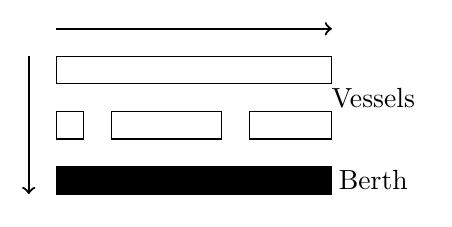
\begin{tikzpicture}[scale=0.35]
      \draw[rotate=90,fill=black] (0,0) rectangle (1,10);
      \draw[rotate=90](2,0) rectangle (3,3);
      \draw[rotate=90](2,4) rectangle (3,8);
      \draw[rotate=90](2,9) rectangle (3,10);
      \draw[rotate=90](4,0) rectangle (5,10);

      \draw[thick,->] (-11,5)--(-11,0);
      \draw[thick,->] (-10,6)--(0,6);

      \node at (1.5,0.5) {Berth};
      \node at (1.5,3.5) {Vessels};
    \end{tikzpicture}
    \caption{Example of berth allocation. Vessels are docked in berth locations (horizontal) and are queued over time (vertical). The vertical arrow represents the movement direction of queued vessels and the horizontal arrow represents the direction of departure.}
    \label{subfig:bapexample}
  \end{figure}

  \begin{figure}[htpb]
    \centering
    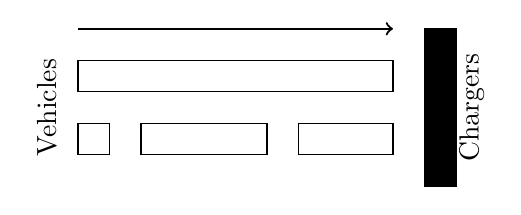
\begin{tikzpicture}[scale=0.4]
      \draw[fill=black] (0,0) rectangle (1,5);

      \draw[rotate=90](1,1) rectangle (2,4);
      \draw[rotate=90](1,5) rectangle (2,9);
      \draw[rotate=90](1,10) rectangle (2,11);
      \draw[rotate=90](3,1) rectangle (4,11);

      \draw[thick,->] (-11,5)--(-1,5);

      \node[rotate=90] at (-12,2.5) {Vehicles};
      \node[rotate=90] at (1.5,2.5) {Chargers};
    \end{tikzpicture}
    \caption{Example of position allocation. Vehicles are placed in queues to be charged and move in the direction indicated by the arrow.}
    \label{subfig:papexample}
  \end{figure}
